\subsection*{\textit{\textbf{RQ1: Are addressed issues delivered more quickly
in rapid releases?}}}

\begin{figure}[t!]
	\centering
	\subfloat[Lifetime]{
		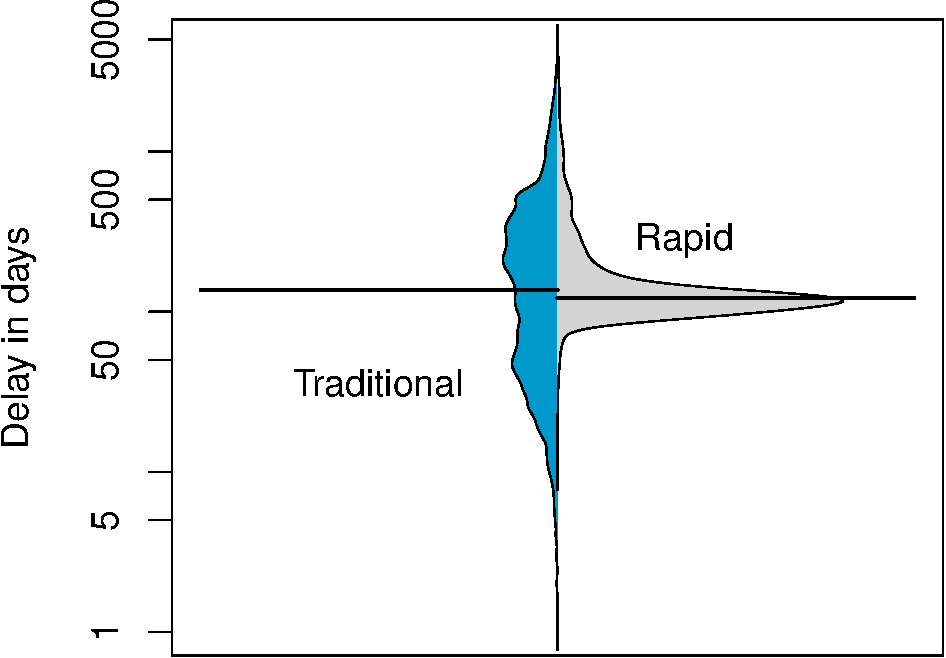
\includegraphics[width=.45\columnwidth,keepaspectratio]
		{chapters/chapter5/figures/rq1/trad-vs-rapid-entire.pdf}
		\label{fig:delivery_delay}
	}
	\subfloat[Triaging phase]{
		\centering
		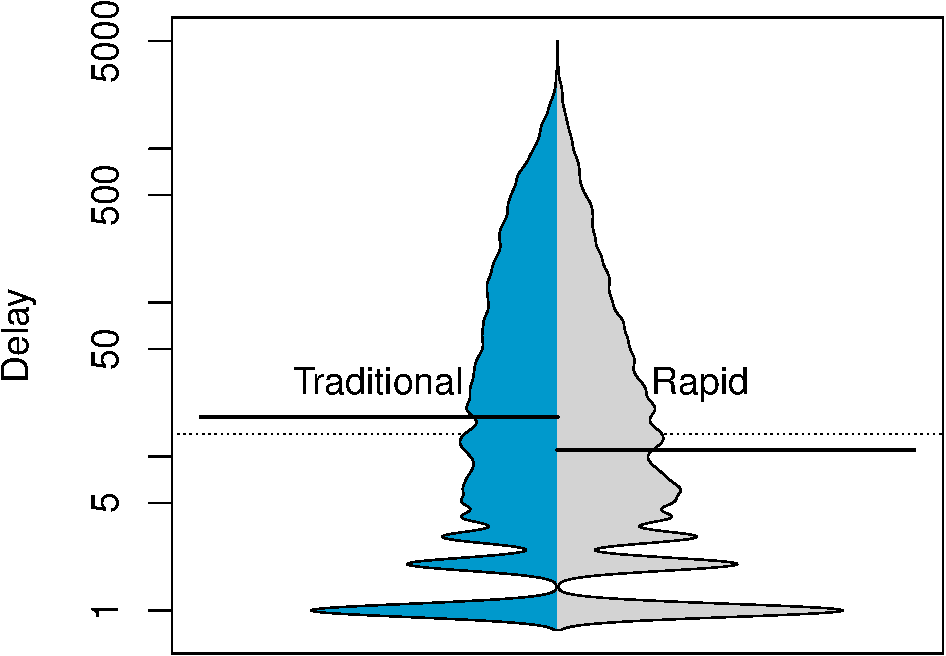
\includegraphics[width=.45\columnwidth,keepaspectratio]
		{chapters/chapter5/figures/rq1/traditional_vs_rapid_triaging.pdf}
		\label{fig:triaging}
	}

	\subfloat[Fixing phase]{
		\centering
		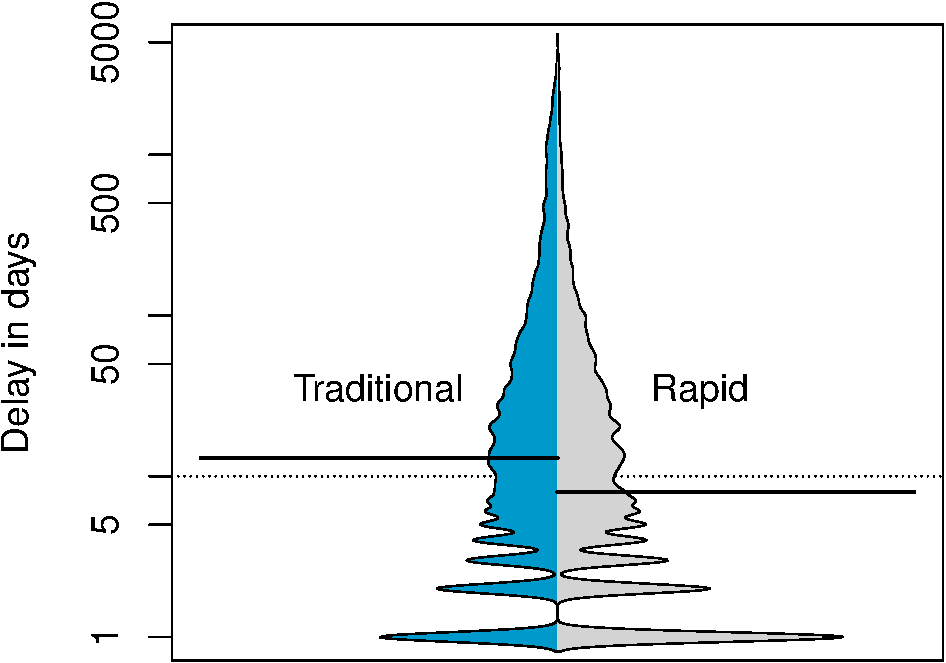
\includegraphics[width=.45\columnwidth,keepaspectratio]
		{chapters/chapter5/figures/rq1/traditional_vs_rapid_fixtime.pdf}
		\label{fig:fixtime}
	}
	\subfloat[Integration phase]{
		\centering
		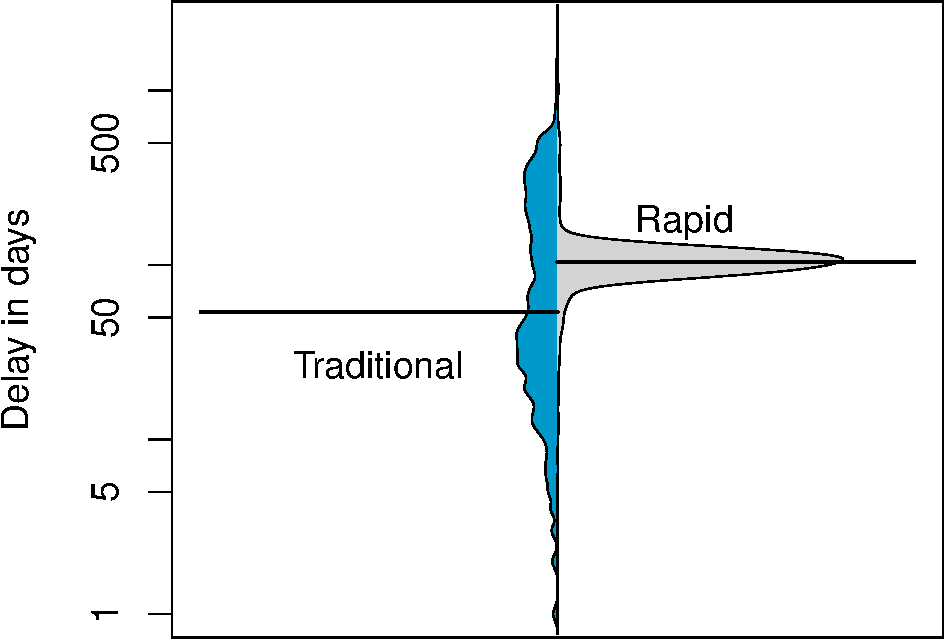
\includegraphics[width=.45\columnwidth,keepaspectratio]
		{chapters/chapter5/figures/rq1/traditional_vs_rapid.pdf}
		\label{fig:traditional_vs_rapid}
	}
	\caption{Time spans of the phases involved in the lifetime of an issue.}
	\label{fig:timespans}
\end{figure}

\noindent\textit{\textbf{Observation~1---There is no significant difference between traditional
and rapid releases regarding issue lifetime.}}\observation{obs:1}
\hyperref[fig:delivery_delay]{Figure}~\ref{fig:delivery_delay} shows the distributions of the lifetime of the
issues in traditional and rapid releases. We observe a $p<1.03e^{-14}$ but a
$negligible$ difference between the distributions ($\textit{delta}=0.03$). We
also observe that traditional releases have a greater MAD ($154$ days) than
rapid releases ($29$ days), which indicates that rapid releases are more
consistent with respect to the lifetime of the issues. Our results indicate that
the difference in the issues' lifetime between traditional and rapid releases is
not as obvious as one might expect. We then look at the triaging, fixing, and
integration time spans to better understand the differences between traditional
and rapid releases.\\

\noindent\textit{\textbf{Observation~2---Addressed issues are triaged and fixed more quickly in
rapid releases, but tend to wait for a longer time before being
delivered.}}\observation{obs:2}
\hyperref[fig:triaging]{Figures}~\ref{fig:triaging}~,~\ref{fig:fixtime},~and~\ref{fig:traditional_vs_rapid}
show the triaging, fixing, and integration time spans, respectively. We observe
that addressed issues take a median time of 54 days to be integrated into
traditional releases, while taking 104 days (median) to be integrated into rapid
releases. We observe a $p<2.2e^{-16}$ with a $small$ effect-size
($delta=-0.25$).

Regarding fixing time span, an issue takes 6 days (median) to be fixed in
rapid releases, and 9 days (median) in traditional releases. These results
are statistically significant $p<2.2e^{-16}$, but there is only a $negligible$
difference between distributions ($delta=0.13$). 

Our results complement previous research. Khomh~\etal \cite{khomh2012faster}
found that post- and pre-release bugs that are associated with crash reports are
fixed faster in rapid Firefox releases than in traditional releases.
Furthermore, we observe a significant $p<2.2e^{-16}$ but $negligible$
difference ($\textit{delta}=0.11$) between traditional and rapid releases
regarding triaging time. The median triaging time for rapid and traditional
releases are 11 and 18 days, respectively.

When we consider both pre-integration phases together (triaging $t1$ plus
fixing $t2$ in \hyperref[fig:issue_lifecycle]{Figure}~\ref{fig:issue_lifecycle}), we observe that an issue takes
$11$ days (median) to triage and address in rapid releases, while
it takes $19$ days (median) in traditional releases. We observe a $p<2.2e^{-16}$ with a $small$
effect-size ($delta=0.15$). Our results suggest that even though issues have
shorter pre-integration phases in rapid releases, they remain ``on the
shelf'' for a longer time on average.

Finally, we again observe that rapid releases are more consistent than
traditional releases in terms of fixing and integration rate. Rapid releases
achieve MADs of 9 and 17 days for fixing and integration, respectively. The
values for traditional releases are 13 and 64 days for fixing and integration,
respectively.\\ 

\conclusionbox{Although issues are triaged and fixed faster in rapid releases,
they tend to take a longer time to be integrated. However, the delivery rate
of addressed issues is more consistent in rapid releases than in traditional
ones.}

